\documentclass[tikz,border=0.1cm]{standalone}

\definecolor{Orange}{HTML}{fa7303}
\definecolor{Blue}{HTML}{0e0441}

\begin{document}

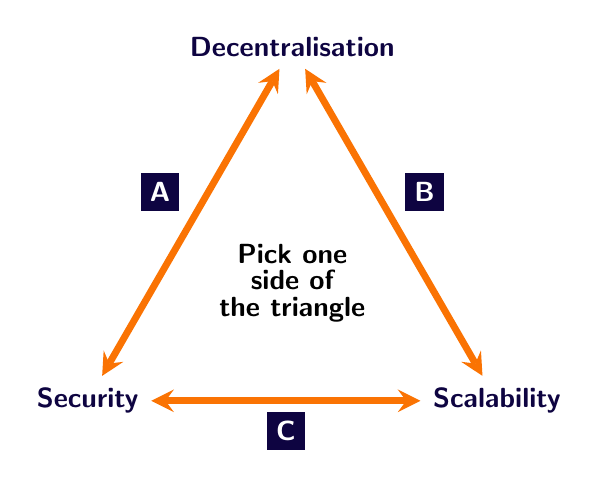
\begin{tikzpicture}[>=stealth,line width=2.5pt,
n/.style={text=white,fill=#1,midway},
nodes={font=\bfseries\sffamily}]
\renewcommand{\baselinestretch}{.8} 
\def\r{3} 
\path[nodes={align=center}]
(0,0) node{Pick one\\side of\\the triangle}
(90:\r) node (C) {\textcolor{Blue}{Decentralisation}}       
(210:\r) node (B) {\textcolor{Blue}{Security}}
(-30:\r) node (A) {\textcolor{Blue}{Scalability}}
;
\draw[<->,Orange] (A)--(B) node[n=Blue,below=1mm]{C};
\draw[<->,Orange] (B)--(C) node[n=Blue,above left=1mm]{A};
\draw[<->,Orange] (C)--(A) node[n=Blue,above right=1mm]{B};
\end{tikzpicture}   


\end{document}